% The master copy of this demo dissertation is held on my filespace
% on the cl file serve (/homes/mr/teaching/demodissert/)

% Last updated by MR on 2 August 2001

\documentclass[12pt,twoside,notitlepage]{report}

\usepackage{a4}
\usepackage{verbatim}
\usepackage{amsmath}
\usepackage{amssymb}
\usepackage{amsthm}
\usepackage{setspace}
\usepackage{longtable}
\usepackage{pdfpages}
\usepackage{graphicx}
\usepackage{amscd}



\input{epsf}                            % to allow postscript inclusions
% On thor and CUS read top of file:
%     /opt/TeX/lib/texmf/tex/dvips/epsf.sty
% On CL machines read:
%     /usr/lib/tex/macros/dvips/epsf.tex



\raggedbottom                           % try to avoid widows and orphans
\sloppy
\clubpenalty1000%
\widowpenalty1000%

\addtolength{\oddsidemargin}{6mm}       % adjust margins
\addtolength{\evensidemargin}{-8mm}

\renewcommand{\baselinestretch}{1.3}    % adjust line spacing to make
                                        % more readable

\begin{document}

\bibliographystyle{plain}


%%%%%%%%%%%%%%%%%%%%%%%%%%%%%%%%%%%%%%%%%%%%%%%%%%%%%%%%%%%%%%%%%%%%%%%%
% Title


\pagestyle{empty}

%\hfill{\LARGE \bf Martin Richards}

\vspace*{60mm}
\begin{center}
\Huge
{\bf An Exact Real Package in ML} \\
\vspace*{5mm}
Shi Shu \\
\vspace*{5mm}
Fitzwilliam College \\
\vspace*{5mm}
\today  % today's date
\end{center}

\cleardoublepage

%%%%%%%%%%%%%%%%%%%%%%%%%%%%%%%%%%%%%%%%%%%%%%%%%%%%%%%%%%%%%%%%%%%%%%%%%%%%%%
% Proforma, table of contents and list of figures

\setcounter{page}{1}
\pagenumbering{roman}
\pagestyle{plain}

\chapter*{Proforma}

{\large
\begin{tabular}{ll}
Name:               & \bf Shi Shu                       \\
College:            & \bf Fitzwilliam College                     \\
Project Title:      & \bf An Exreal Package in ML 	\\
Word Count:         & \bf 9371 \\
Project Originator: & Dr. Arno~Pauly                    \\
Supervisor:         & Dr. Arno~Pauly                     \\ 
\end{tabular}
}
%\footnotetext[1]{This word count was computed
%by {\tt detex diss.tex | tr -cd '0-9A-Za-z $\tt\backslash$n' | wc -w}
%}
%\stepcounter{footnote}


\section*{Original Aims of the Project}

The project mainly focuses on building an exact real package and basic arithmetic on the datatype in ML. And then evaluate its performance and comparing it with other exact real implementations such as iRRAM. Then implement mathematical concept such as open/closed set on real numbers and real intervals on developed data structure. Then completing the algorithm of the inverse function calculator using the package will be an extension to the project. 


\section*{Work Completed}

I did research on many of the well developed ways of representing real numbers and choose one representation to implement the exact real number datatype. Basic arithmetic operation is implemented for the developed datatype. And also an inverse function calculator is implemented using the Exreal datatype constructed. The performance of the constructed datatypes and functions is evaluated both theoretically and empirically.

\section*{Special Difficulties}
None
 
\newpage
\section*{Declaration}

I, Shi Shu of Fitzwilliam College, being a candidate for Part II of the Computer
Science Tripos, hereby declare
that this dissertation and the work described in it are my own work,
unaided except as may be specified below, and that the dissertation
does not contain material that has already been used to any substantial
extent for a comparable purpose.

\bigskip
\leftline{Signed [signature]}

\medskip
\leftline{Date [date]}

\cleardoublepage

\tableofcontents

\newpage
\section*{Acknowledgements}

Thanks to my supervisor Arno Pauly for useful supervisions and helpful advices on the dissertation. 

%%%%%%%%%%%%%%%%%%%%%%%%%%%%%%%%%%%%%%%%%%%%%%%%%%%%%%%%%%%%%%%%%%%%%%%
% now for the chapters

\cleardoublepage        % just to make sure before the page numbering
                        % is changed

\setcounter{page}{1}
\pagenumbering{arabic}
\pagestyle{headings}

\chapter{Introduction}

\section{Motivation}

Many applications of computers require the use of real arithmetic. Unfortunately, there are a number of significant problems associated with performing real arithmetic using floating point approximation, the method most commonly used by programmers, and which forms part of most computer languages and the instruction set of many modern CPUs. These problems stem from the fact that only a finite set of reals are represented exactly using this approach, and rounding occurs after each floating point operation. And the accumulation of rounding errors can lead to highly inaccurate results. They can result in complete loss of accuracy in even relatively simple computations. The exact real datatype would allow us to give a precise representation for any real number and do calculation without rounding error.



\section{Related Work}



\subsection {Exact Real Arithmetic Systems Competition}
A competition between systems for doing exact real number computations was held in September 2000 \cite{blanck}. They tested the ability of three major exact real number systems at the time in term of performing calculatation like the square root of $\pi$. The three major system that were tested are :\\
\begin{itemize}
\item \textbf{MAP} Manchester Arithmetic Package
\item \textbf{iRRAM} Iterative Real RAM package in C++
\item \textbf{MPFR} Multiple-precision floating-point computations with correct rounding Library in C\cite{mpfr}.
\end{itemize}

The test result indicates that in most scenorios, the iRRAM package in C++ had the best performance.


\subsection{iRRAM}
The iRRAM is a C++ package for error-free real arithmetic based on the concept of a Real-RAM\cite{irram}. Its capabilities range from ordinary arithmetic over trigonometric functions to linear algebra and even differential equations.\\
A program for the iRRAM is coded in ordinary C++, but may use a special class REAL, that behaves like real numbers without any error. A quite small set of operations is allowed to be used directly with variables of this type: usual arithmetic operations, tests and conversion to/from integer or other types. Programmer can use other programming methods from C++, like defining own data types.

\subsection {Different focus of this project}
Most of the previous exact real packages developed in different languages focus on developing arithmetic functions over the data structure. Many of these packages focus on implementing effective ways of calculating functions such as logarithms and trigonometry etc. While this project focus on developing a package of exact real number using a fundamentally functional approach. Along with basic arithmetic, many other data structures based on the real representation are introduced here as well, such as \emph{open set}, \emph{closed set}, \emph{compact set} on reals and real intervals etc. Also by utilising the admissibility of the chosen real representation and these developed data structure, a function inverse calculator is implemented.  



\section {Project Goals}


\begin{itemize}
\item Find a proper representation of real number and implement the data structure in ML.
\item Implement the basic arithmetic using the developed data structure.
\item Implement related mathematical concepts such as \emph{open/closed set, compact set} on real number and real intervals.
\item Implement an inverse function calculator using the developed exact real number data type. 
\end{itemize}



\cleardoublepage



\chapter{Preparation}

\section {Choice of Real Representation}

Since floating point has been proved to be not sufficient under many situations, Exact real representations are mostly based on infinite data streams. Here I introduce three of the commonly used exact real representations.  
\subsection {Real Representation and real number function}



\textbf{Definition 2.1 (Representation)} \cite{weihrauchd} \\
A representation of the real numbers $\mathbb{R}$ is a surjective function: 

\begin{equation}
\delta : \subseteq \Sigma^{\omega} \rightarrow \mathbb{R}
\end{equation}\\
Here $\Sigma^{\omega}$ denotes the set of infinite sequences over the alphabet $\Sigma$, the inclusion symbol $\subseteq$ indicates a potentially partial functions. An example of a representation is the ordinary decimal representation.\\
\textbf{Definition 2.2 (Computable real number function)} \cite{weihrauchd}\\
A function $\textit{f}  : \subseteq \mathbb{R} \rightarrow \mathbb{R}$ is called computable with respect to some representation $\delta : \subseteq \Sigma^{\omega} \rightarrow \mathbb{R}$, if there exists some Turing machine $M$ with one-way output tape which computes infinitely long and which in the long run transforms each sequence $p\in\Sigma^{\omega}$ which represents some $x:=\delta(p)\in \mathbb{R}$ into some sequence $q\in\Sigma^{\omega}$ which represents $f(x)$ , i.e. $f(x)=\delta(q)$ .\\

With these definitions, we can see why ordinary decimal representation is not sufficient in some cases. For example, multiplication by 3, $i.e$ . the real function $f$ : $\mathbb{R} \rightarrow \mathbb{R},$ $x \rightarrow 3x$ is not computable with respect to the decimal representation \cite{peter}.\\ To show $3x$ is not computable is quite easy: each machine which would compute multi- plication by 3 w.r.t. the decimal representation has to transform the input $p=0.33333\ldots$ or to either to $q=$ 0.9999.... or to $q^{'}=$ 1.0000.... Especially, the machine has to write 0.9 or 1.0 on the output tape after some finite time, but no finite prefix of the input sequence $p$ suffices to decide whether the correct output sequence has to start with 0.9 or with 1.0. Consequently, such a machine cannot exist.\\
Thus other representations of real numbers are introduced.

\subsection {Sequence of Interval Representation}
\textbf{Definition 2.3 (Sequence of Interval Representation)}\cite{weihrauchd}\\
Define $\rho _{\textit{I}}: \subseteq \Sigma^{\omega} \rightarrow \mathbb{R}$ as follows :

\begin{equation}
\begin{split}
\rho _{\textit{I}} (p) = \textit{x} \mbox{ , if and only if there are }u_{0} , v_{0} , u_{1} v_{1} .... \in \mathbb{Q} \\
\mbox{ with } p = [u_{\textit{0}} , v_{\textit{0}}],[u_{\textit{1}} , v_{\textit{1}}], ...... \mbox{ and } \textit{x} = sup(u_{\textit{i}}) = inf(v_{\textit{i}})\\
\end{split}
\end{equation}\\
With this representation, basic arithmetic can be easily implemented, basically doing rational arithmetic on all the end point of all the intervals. Thus initially it would seem to be a nice representation to implement, but this implementation would have a very high memory requirement for every single exreal. Even utilising the laziness of ML, each real number would require at least 2 rational numbers to a rather high precision. Hence this representation is far from ideal for computer implementation.
\subsection {Cauchy Representation}
\textbf{Definition 2.4 (Cauchy Representation)}\cite{weihrauchd}\\
Define $\rho _{\textit{C}}: \subseteq \Sigma^{\omega} \rightarrow \mathbb{R}$ as follows :

\begin{equation}
\begin{split}
\rho _{\textit{C}} (p) = \textit{x} \mbox{ , if and only if there are }u_{0} , u_{1} , u_{2} .... \in \mathbb{Q} \\
\mbox{ with } p = u_{0}|u_{1}|u_{2}....  \mbox{ and } \\
\forall k \mbox{ } \forall \textit{i} >k \mbox{ } |u_{\textit{i}}-u_{\textit{k}}| < 2^{-k} \mbox{ and } \textit{x} = \lim_{\textit{i}\to\infty} u_{\textit{i}} 
\end{split}
\end{equation}\\
This representation is equivalent to the sequence of interval representation (proof can be found here \cite{weihrauchd}) and with a minimal guaranteed converging speed. Thus the space usage problem remains for computer implementation. 


\subsection {Signed Digit Representation}
\textbf{Definition 2.5 (Signed Digit Representation)}\cite{weihrauchd}\\
Define $\rho _{\textit{S}}: \subseteq \Sigma^{\omega} \rightarrow \mathbb{R}$ as follows :

\begin{equation}
\begin{split}
\rho _{\textit{S}} (p) = \textit{x} \\
\mbox{if and only if there are } u_{1} , u_{2} , u_{3}.... \mbox{and } v_{1} , v_{2} , v_{3} ...v_{m} \in \{1,0,-1\}  \\
\mbox{ with } p = v_{m}v_{m-1}...v_{2}v_{1}.u_{1}u_{2}u_{3}....  \mbox{ and } \\
\textit{x} = \sum_{i=1}^{m} 2^i*v_{i} +  + \sum_{i=1}^{\infty} 2^{-i}*u_{i} 
\end{split}
\end{equation}\\

Signed digit representation is defined like the decimal representation but which also allows negative digits.  Most concrete continuous functions which are used in analysis are computable in this sense. The actual implementation can work as a proof for addition and multiplication.\\
\textbf{Theorem 2.1} (\textbf{Undecidability of the equality}) \\
The equality test on the real numbers is not decidable, $i.e$ . the function
\begin{equation}
s : \mathbb{R}^{2} \rightarrow \mathbb{R},
(x, y)\mapsto 
\begin{cases}
0& \text{if \textit{x} = \textit{y}}\\
1& \text{else}
\end{cases}
\end{equation}\\
is not computable\cite{peter}.
The undecidability of the equality is not a bad property of the signed-digit representation (in the sense as the non-computability of the multiplication by 3 is a bad property of the decimal representation). Unfortunately equality is undecidable with respect to all representations of the real numbers. In other words: there is no way to represent real numbers which could enable physical computers to decide equality and that make the next data type introduced crucial in our implementation.

\section {Sierpinski Space}
In mathematics, the Sierpinski space (or the connected two-point set) is a finite topological space with two points, only one of which is closed. \\
The Sierpinski space is a topological space defined as 
\begin{itemize}
\item The underlying set is a two-point set $\textit{S}$ $=$ \{ $\top$,$\bot$ \}. 
\item The open subsets are  \{\} , \{$\bot$\}, \{$\top$,$\bot$\} , the closed subset are \{\}, \{$\top$\}, \{$\top$, $\bot$\}.
\end{itemize}
~\\
Based on the definition we can consider $\top$ (or true) as the "observable true" and $\bot$ as "unobservable
false". 
Sierpinski Space is then used in place of boolean in the developed real number systems. Due to the undecidability of inequality between real numbers, we use this semi decidable data structure to implement the undecidable not-equality of real numbers.




\section {Topology}
\subsection {Open Sets}
\textbf{Definition 2.6} \cite{john}\\
A set \textit{G} $\subset$ $\mathbb{R}$ is open if for every $\textit {x}$ $\in$ $\textit {G}$ there exist a $\delta$ $>$ 0 such that $\textit {G}$ $\supset$ ($\textit {x-$\delta$, x+$\delta$}$) . For every open set, a characteristic function can defined as :
\begin{equation}
C : \mathbb{R} \rightarrow \mbox{Boolean },
\textit{x} \mapsto 
\begin{cases}
\text{true}& \text{if \textit{x} is in the open set}\\
\text{false}& \text{else}
\end{cases}
\end{equation}\\
\textbf{Theorem 2.2} An arbitrary union of open sets is open, and a finite intersection of open sets is open.\\
Here we introduced the idea of \emph{synthetic topology} \cite{escardo} for implementation purpose. In synthetic topology we define the open set as,\\
\textbf{Definition 2.7} \cite{escardo} A subset U of a data type $a$ is called open if its characteristic function $f_U : a \to$ Sierpinski Space defined by $f_U(x) = \top$ if and only if $x \in U$ is continuous. 

\subsection {Closed Sets}
\textbf{Definition 2.8} A set \textit{F} $\subset$ $\mathbb{R}$ is closed if $\textit{F} ^{c}$ $=$ \{ $\textit {x}$ $\in$ $\mathbb{R}$ $:$ $\textit {x}$ $\notin$  \textit{F} \} is open. \\
\textbf{Theorem 2.3} An arbitrary intersection of closed sets is closed, and a finite union of closed sets is closed.\\
The implementation of open/closed set on exact real number in \textbf{Section 3.3} can show that any countable unions/intersections of open sets is an open set and any countable unions/intersections of closed sets is a closed set.
 
\subsection {Compact Sets}
There are different ways of defining \emph{compact set}.\\
\textbf{Definition 2.9 Sequential Definition} \cite{john}\\
A set $K \subset \mathbb{R}$ is sequentially compact if every sequence in $K$ has a convergent subsequence whose limit belongs to $K$.\\

Intuitively, a compact set confines every sequence of points in the set so much that the sequence must accumulate at some point of the set. \\
\textbf{Definition 2.10 Topological Definition} \cite{john}\\
Let A $\subset$ R. A cover of A is a collection of sets $\{ A_i \subset \mathbb{R} : i \in I\}$ whose union contains A,\\
\begin{equation}
\bigcup_{i \in I} A_i \supset A
\end{equation}\\
An open cover of A is a cover such that $A_i$ is open for every $i \in I$.\\
Suppose that $C =\{A_i \subset R : i \in I\}$ is a cover of $A$ $\subset$ $R$. \\
A subcover $S$ of $C$ is a sub-collection $S \subset C$ that covers $A$, meaning that\\ 
\begin{equation}
S = \{A_{i_k} \in C : k \in J\},  \bigcup_{k \in J} A_{i_k} \supset A
\end{equation}\\
A finite subcover is a subcover $\{A_{i_1}, A_{i_2},...,A_{i_n}\}$ that consists of finitely many sets.\\
Then we define a set $K$ $\subset$ $R$ to be compact if every open cover of $K$ has a finite subcover.\\

Also for implementation purpose, a synthetic approach to define \emph{compact sets} is introduced as following \cite{escardo},\\
\textbf{Definition 2.11} \cite{escardo}\\
We call a subspace $Q$ of a data type $a$ compact if its universal quantification function $\forall_{Q} : (a \to Sierpinski Space) \to Sierpinski Space$ defined by\\
$\forall_{Q}(p) = \top$ if and only if $p(x) = \top$ for all $x \in Q$ is continuous. Here $p$ is an arbitrary predicate function that has the type $p : a \to Sierpinski Space$.\\

Definition 2.11 is equivalent to Definition 2.10. The reason that the sequential compactness can not be used here is that it does not give rise to a computable type \cite{gherardi4}.\\
\textbf{Theorem 2.4} The intersection of a compact set and a closed set is a compact set.\\
It is proven in \textit{On the topological aspects of the theory of represented spaces} Proposition 11.4 by Arno Pauly \cite{pauly-synthetic-arxiv}. 


\section {Admissibility}
\textbf{Definition 2.12 Admissimility} \\
Let $\delta_\mathbf{X} : \Sigma^\omega \to \mathbf{X}$ and $\delta_\mathbf{Y} : \Sigma^\omega \to \mathbf{Y}$ be representations on $\mathbf{X}$ and $\mathbf{Y}$. Here $\mathbf{X}$ and $\mathbf{Y}$ are topological spaces. $\delta_\mathbf{Y}$ is an admissible representation if and only if for any continuous function $f: \mathbf{X} \to \mathbf{Y}$, there exist a continuous function $F : \Sigma^\omega \to \Sigma^\omega$ such that  it makes the following diagram commutes.

$$\begin{CD}
\Sigma^\omega @>F>> \Sigma^\omega\\
@VV\delta_\mathbf{X}V @VV\delta_\mathbf{Y}V\\
\mathbf{X} @>f>> \mathbf{Y}
\end{CD}$$

One equivalent definition is for any singleton compact set under $\delta_\mathbf{X}$ representation, the function $f = \{\mathbf{x}\} \to \mathbf{x} : Compact(\mathbf{X}) \to \mathbf{X}$ is computable. Then $\delta_\mathbf{X}$ is an admissible representation. 
 

The signed digit representation of real number is an admissible representation of real numbers \cite{weihrauchd}. An algorithm of how to use admissibility can be described as below \cite{pauly-synthetic-arxiv},


\begin{itemize}
\item Conclude that the solution set S is closed based on its definition.
\item Obtain some compact candidate set K (either from the situation, or by assumption - this often involves some bounds).
\item Compute $Intersect(S,K)$ as a compact set via \textbf{Theorem 2.4}.
\item Use domain-specific reasoning or assumption to conclude that the solution s is unique.
\item As we have singleton \{s\} available as a compact set, if our target space is admissible, we can compute s.
\end{itemize}

This work as our key algorithm to implement the inverse function calculator.


\section {Software Development Approach}
\subsection {Development Environment}
The development and testing environment is in Mac OS X 10.10 with 2GHz Intel Core i7 CPU and 8GB 1600 MHz DDR3 memory. 
\subsection {Programming Language and Software}
ML is the choice of language here since many infinite data structure such as Exreal and Sierpinski Space will be implemented and the laziness that ML provide us with easy evaluation of these data structure.\\
Among different versions of ML available, Poly/ML is used here. Poly/ML was originally written by David Matthews at the Computer Laboratory at Cambridge University.  It was written in an experimental language, Poly, similar to ML but with a different type system. The current version 4.0 release Poly/ML supports the full version of the language as given in the "Definition of Standard ML (Revised)", generally known as ML97. \cite{poly} \\
During the testing phase, New Jersey ML \cite{njml} is also tried for performance comparison and no significant difference is noticed.

\subsection {Back Up}
Code and Dissertation are backed up using both Dropbox and physical external hard drive.
\subsection {Extendability of the code}
For easier later expansion and possible comparison, most functions that work on exreal (except basic arithmetic) are independent of the representation of the exact real numbers. Thus if another representation of real number is implemented then most of the code would still be usable on the new representation with minimal modification.



\cleardoublepage
\chapter{Implementation}



\section{Real Representation}


\subsection{Exreal Datatype}

Among many representations of real numbers, signed binary representation is used here.
Real number are resented by a regular integer and a lazy list of signed binaries, which consist of \{1,0,-1\}.

{\setstretch{0.8}
\begin{verbatim}
datatype 'a seq = Cons of 'a * (unit -> 'a seq);
datatype exreal = R of int * int seq;
\end{verbatim}
}

Here we assume that all real numbers have a infinitely long fraction part. We write finite length real number (rationals) such as 0.75 as :

{\setstretch{0.8}
\begin{verbatim}
> fun zeros () = Cons(0,fn ()=>zeros ());
val zeros = fn: unit -> int seq
> val rational = (R(0,Cons(1,fn ()=>(Cons(1,fn ()=>zeros())))));
val rational = R (0, Cons (1, fn)): exreal
\end{verbatim}
}



\subsection{Conversion Between real and Exreal}

To allow the easy conversion, conversion function between reals and exreals are introduced.
Thus user can built in real as input, convert it into exreal and after certain operations, convert back to real and return a real number result as expected. \\
From exreal to real, we need user to input a exreal and an integer which indicates how many bits in the lazy list of fractions it requires.

{\setstretch{0.8}
\begin{verbatim}
fun ll2r _ 0 _ = 0.0
|   ll2r (Cons(x,xq)) n i = 
(Real.fromInt(x)/(Math.pow(2.0,i))) + (ll2r (xq()) (n-1) (i+1.0));
val ll2r = fn: int seq -> int -> real -> real
fun exr2r (R(i,f)) n = Real.fromInt(i)+(ll2r f n 1.0);
val exr2r = fn: exreal -> int -> real
\end{verbatim}
}
    
On the other hand, from real number to exreal, first change the real into binary to the desired precision. Then an integer sequence filled with 0s is attached to the tail to make the returned result exreal.

{\setstretch{0.8}
\begin{verbatim}
fun r2ll x 0 i = zeros()
|   r2ll x n i = if Real.signBit(x - 1.0/Math.pow(2.0,i)) 
      then Cons(0,fn ()=> r2ll x (n-1) (i+1.0))
      else Cons(1, fn ()=> r2ll (x- 1.0/Math.pow(2.0,i)) (n-1) (i+1.0)); 
val r2ll = fn: real -> int -> real -> int seq
fun r2exr r n = (R(floor r, r2ll (r - Real.fromInt(floor r)) (n) (1.0)));
val r2exr = fn: real -> int -> exreal
\end{verbatim}
}

A simple conversion example as shown below :
{\setstretch{0.8}
\begin{verbatim}
> val test = r2exr 2.3 100;
val test = R (2, Cons (0, fn)): exreal
> exr2r test 5;
val it = 2.28125: real
> exr2r test 10;
val it = 2.299804688: real
> exr2r test 100;
val it = 2.3: real
\end{verbatim}
}



 
\subsection{Addition}
In exreal addition, the importance of having the signed binary representation instead of standard binary can be shown. In exact real arithmetic, the major difficulty would be calculation needs to be done from left to right. And bits needs to be determined without allowing the carryovers from following bits to affect this bit.\\
To add two exreal numbers, first we add the two integer and the two lazy list correspondingly. The bitwise addition of two fraction part of exreals has a result of a lazy list consist of \{2,1,0,-1,-2\}.

{\setstretch{0.8}
\begin{verbatim}
> fun frac_sum1 (Cons(x,xq),Cons(y,yq)) = 
      Cons(x+y,fn ()=>(frac_sum1(xq(),yq())));
val frac_sum1 = fn: int seq * int seq -> int seq
\end{verbatim}
}

Then evaluation of the result lazy list is required.\\
To determined the current bit, two further bits would be required to be evaluated. By examining the third bit, possible carryovers from the third bit to the second bit can be determined. Then with the possible carryovers from the third bit and current second bit, the possible carryovers from the second bit to current bit can be determined.  And then the signed binary representation will help to eliminate the possible carryover to the current bit. For example, we have a sequence of 011... then the third bit is 1 and thus the possible carryover to the second bit is [0,1]. Since the second bit is currently one and with the possible carryover [0,1], thus second bit has a possible carry over of [0,1] to the current bit. Then we can set second bit to -1 and set the current bit to 1 to avoid any possible carryovers to the current bit. Then recursively evaluate the sequence -11.... It seems to have $5^{3}=125$ possibilities. But in reality many of can never occur due to the pre-evaluation.  All possible different situation can be listed as below.\\

\begin{longtable}{| l | l | l | l |}
	\hline
    	Current Bit & Next 2 Bits & Possible Carryover & Evaluated Result \\ \hline
	1 & 2, \_ & 1 & 0, 0, ...\\ \hline
	1 & 1,0 & 0 & 1, 1, ...\\ \hline
	1 & 1,-1 & 0 & 1, 1, ...\\ \hline
	1 & 1,-2 & 0 & 1, 1, ...\\ \hline	
	1 & 1,1 & 0,1 & 0, -1, ...\\ \hline
	1 & 1,2 & 1 & 0, -1, ...\\ \hline
	1 & 0,\_ & 0 & 1, 0, ...\\ \hline
	1 & -1,-1 & 0,-1 & 0, 1, ...\\ \hline
	1 & -1,-2 & 0,-1 & 0, 1, ...\\ \hline
	1 & -1,0 & 0 & 1, -1, ...\\ \hline
	1 & -1,1 & 0 & 1, -1, ...\\ \hline
	1 & -1,2 & 0 & 1, -1, ...\\ \hline
	1 & -2,\_ & -1 & 0, 0, ...\\ \hline
	0 & 2,\_ & 1 & 1, 0, ...\\ \hline
	0 & 1,2 & 1 & 1, -1, ...\\ \hline
	0 & 1,1 & 0,1 & 1, -1, ...\\ \hline
	0 & 1,-2 & 0 & 0, 1, ...\\ \hline
	0 & 1,-1 & 0 & 0, 1, ...\\ \hline
	0 & 1,0 & 0 & 0, 1, ...\\ \hline
	0 & 0,\_ & 0 & 0, 0, ...\\ \hline
	0 & -1,-2 & -1 & -1, 1, ...\\ \hline
	0 & -1,-1 & 0,-1 & -1, 1, ...\\ \hline
	0 & -1,2 & 0 & 0, -1, ...\\ \hline
	0 & -1,1 & 0 & 0, -1, ...\\ \hline
	0 & -1,0 & 0 & 0, -1, ...\\ \hline
	0 & -2,\_ & -1 & -1, 0, ...\\ \hline
	-1 & 2,\_ & -1 & 0, 0, ...\\ \hline
	-1 & 2,\_ & 1 & 0, 0, ...\\ \hline
	-1 & 1,1 & 0,1 & 0, -1, ...\\ \hline
	-1 & 1,2 & 1 & 0, -1, ...\\ \hline
	-1 & 1,0 & 0 & -1, 1, ...\\ \hline
	-1 & 1,1 & 0 & -1, 1, ...\\ \hline
	-1 & 1,2 & 0 & -1, 1, ...\\ \hline
	-1 & 0,\_ & 0 & -1, 0, ...\\ \hline
	-1 & -1,-1 & 0,-1 & 0, 1, ...\\ \hline
	-1 & -1,-2 & -1 & 0, 1, ...\\ \hline
	-1 & -1,0 & 0 & -1, -1, ...\\ \hline
	-1 & -1,1 & 0 & -1, -1, ...\\ \hline
	-1 & -1,2 & 0 & -1, -1, ...\\ \hline

\end{longtable}

Then combining the result of the evaluation and the integer addition by adding/subtracting the carryover from the first bit to the integer part. Exreal addition can be integrated as,

{\setstretch{0.8}
\begin{verbatim}
> fun rplus (R(x1,y1)) (R(x2,y2)) = 
     let val temp = frac_sum1(y1,y2) in 
        if head(temp) = 2 
        orelse (take(2,temp)=[1,2] 
        orelse (take(3,temp)=[1,1,1] 
        orelse take(3,temp)=[1,1,2])) 
        then (R(x1+x2+1,eval_result (temp)))
   
        else if head(temp) = ~2 
        orelse (take(2,temp)=[~1,~2] 
        orelse (take(3,temp)=[~1,~1,~1] 
        orelse take(3,temp)=[~1,~1,~2])) 
        then (R(x1+x2-1,eval_result (temp)))
   
        else (R(x1+x2,eval_result(temp)))
     end;
val rplus = fn: exreal -> exreal -> exreal
\end{verbatim}
}

Also addition of a list of exreals is also implemented for the ease of implementing multiplication.





\subsection{Multiplication}
Multiplication can be divided into addition of 4 components. Let's say we want to multiply A and B. Let $A=(R(int1,frac1))$ and $B=(R(int2,frac2))$. Then we have 
\begin{equation}
\begin{split}
A*B=(int1+frac1)*(int2+frac2)\\
=int1*int2+int1*frac2+int2*frac1+frac1*frac2
\end{split}
\end{equation}
The first part of the result is trivial. Two functions need to be implemented is integer multiply with a signed binary lazy list and multiplication between two lazy lists.
To multiply a integer with a lazy list. First convert the integer into a binary form. Let's say that the integer is converted into a $n$ bit binary integer then the multiplication become into the addition of a list of $n$ Exreals. \\
For example, multiplying $10$ and $[1,1,1,1,1,......]$. First , $10$ needs to be converted into $[1,0,1,0]$, which is the binary representation of $10$. Then reverse the result we have $[0,1,0,1]$. Then we have the list of exreals as $[0*R(0,[1,1,1,......]), 1*R(1,[1,1,1,......]), 0*R(3,[1,1,1,......]), 1*R(7,[1,1,1,......])]$. Using Exreal addition implemented in the previous section to add them together, we have the result as $R(9,[1,1,1,......])$.\\
A similar idea is also used for lazy list multiplied with lazy list. First, since the fraction part of an Exreal is within the interval $[-1,1]$ and thus multiply two fraction parts of two Exreal, the result is still in the interval $[-1,1]$. Thus the result still can be represented by a lazy list. \\
Multiply a lazy list $[x_1,x_2,x_3,......]$ with another lazy list y, we have $x_1*[0,y] +x_2*[0,0,y]+x_3* [0,0,0,y]+......$. So the problem become an addition of a lazy list of lazy lists. The difficulty here is to determine how many addition needs to be done to determine the $n^{th}$ bit. From the addition implementation, it can be learned that $(n+1)^{th}$ bit and $(n+2)^{th}$ bit are needed to be examined to determine the $n^{th}$ bit. Thus the $n^{th}$ bit in the result is the $n^{th}$ bit of the result of adding the first $n+2$ elements in generated lazy list.\\
Using (3.1), the Exreal multiplication can be implemented as,

{\setstretch{0.8}
\begin{verbatim}
> fun rmult (R(i1,f1)) (R(i2,f2)) = 
     rplus (R(i1*i2, mult_frac (f1) (f2))) 
          (rplus (mult_frac_int i1 (f2)) (mult_frac_int i2 (f1)));
val rmult = fn: exreal -> exreal -> exreal
\end{verbatim}
}




\section{Sierpinski Space}
The Sierpinski Space is implemented using a lazy list of booleans.
{\setstretch{0.8}
\begin{verbatim}
> datatype Sierpinski = Sierp of bool seq;
\end{verbatim}
}

By using this implementation, the Sierpinski space is $\top$ if and only if there is at least one true in the lazy list. 

{\setstretch{0.8}
\begin{verbatim}
> fun sierp_is_top (Sierp(Cons(x,xq))) = 
     if x = true 
     then true 
     else sierp_is_top (Sierp(xq()));
val sierp_is_top = fn: Sierpinski -> bool
\end{verbatim}
}

This function will not terminate if the Sierpinski Space is bottom, which is false all the time. Thus for testing purposes, the following functions are used for evaluating Sierpinski space, which evaluate the first n entries in the lazy list.

{\setstretch{0.8}
\begin{verbatim}
> fun eval_sierp_aux _ 0 = false 
|     eval_sierp_aux (Cons(true,xq)) n = true
|     eval_sierp_aux (Cons(false,xq)) n = eval_sierp_aux (xq()) (n-1);
val eval_sierp_aux = fn: bool seq -> int -> bool

> fun eval_sierp x n = eval_sierp_aux (sierp_extract_seq(x)) n;
val eval_sierp = fn: Sierpinski -> int -> bool
\end{verbatim}
}

Using the lazy list representation, the OR operation of two Sierpinski Space can be done by interleaving the two lazy list.

{\setstretch{0.8}
\begin{verbatim}
> fun interleave (Cons(x,xf), yq) = Cons(x, fn()=> interleave(yq, xf()));
val interleave = fn: 'a seq * 'a seq -> 'a seq

> fun sierp_or (Sierp(a)) (Sierp(b)) = Sierp(interleave(a,b));
val sierp_or = fn: Sierpinski -> Sierpinski -> Sierpinski
\end{verbatim}
}

The AND operation of two Sierpinski Space A and B can be done by first check the first element of A if it is true then the result Sierpinski Space is B, if not then add a false to the result Sierpinski Space and keep evaluating B and tail(A). Here an easy mistake is to forget to output a false to result at every step, since if both inputs are $\bot$ then the function would keep interleaving between the inputs and give no return. Thus a key thing to keep in mind when implementing functions that return Sierpinski Space as a result, is to make sure the function would make progress at every iteration regardless of the inputs.

{\setstretch{0.8}
\begin{verbatim}
> fun sierp_extract_seq (Sierp(x)) = x;
val sierp_extract_seq = fn: Sierpinski -> bool seq

> fun sierp_and (Sierp(Cons(x,xf))) (Sierp(Cons(y,yf))) = 
     if x=true then (Sierp(Cons(y,yf)))
     else (Sierp(Cons(false,fn ()=> 
          sierp_extract_seq (sierp_and (Sierp(Cons(y,yf))) (Sierp(xf()))))));
val sierp_and = fn: Sierpinski -> Sierpinski -> Sierpinski
\end{verbatim}
}
 
The multiple OR of a lazy list of Sierpinski Space can be done by first checking the first boolean of the first Sierpinski Space of the lazy list if it is true then the result is top or otherwise adding a false to the result and recursively calling it self on the rest of the lazy list and interleaving the result with the tail of the first Sierpinski space in the lazy list. 

{\setstretch{0.8}
\begin{verbatim}
> fun c_true () = Cons(true, fn ()=>c_true());
val c_true = fn: unit -> bool seq

> fun multi_sierp_or (Cons((Sierp(Cons(x,xq))),sf)) = 
     if x = true
     then (Sierp(c_true()))
     else (Sierp(Cons(false, fn()=>
          interleave (sierp_extract_seq(multi_sierp_or (sf())),(xq())))));
val multi_sierp_or = fn: Sierpinski seq -> Sierpinski
\end{verbatim}
}





\section{Open and Closed set on Exreal}

Both \emph{open set} and \emph{closed set} are defined by their characteristic functions. Here a function that takes an input of type $a'$ and returns a Sierpinski Space can be considered as a characteristic function of an open/closed set on type $a'$.
Thus the datatype open and closed set can be defined as,

{\setstretch{0.8}
\begin{verbatim}
> datatype 'a opens = cfo of ('a -> Sierpinski);

> datatype 'a closed = cfc of ('a -> Sierpinski);
\end{verbatim}
}

This implementation allows finding the compliment of an open/closed set to become trivial.

{\setstretch{0.8}
\begin{verbatim}
> fun complementc (cfc(x)) = (cfo(x));
val complementc = fn: 'a closed -> 'a opens

> fun complemento (cfo(x)) = (cfc(x));
val complemento = fn: 'a opens -> 'a closed
\end{verbatim}
}

The UNION of two open sets with characteristic function $f_1$ and $f_2$ can be implemented by using the function
\begin{equation}
f(x) = Sierpinski_{OR} (f_1(x),f_2(x))
\end{equation}
as the characteristic function of the result open set. Similarily INTERSECTION can be done by using
\begin{equation}
f(x) = Sierpinski_{AND} (f_1(x),f_2(x))
\end{equation}
as the characteristic function of the result open set.\\
{\setstretch{0.8}
\begin{verbatim}
> fun opens_union (cfo(x)) (cfo(y)) = 
     cfo (fn a => (sierp_or (x a) (y a)));
val opens_union = fn: 'a opens -> 'a opens -> 'a opens

> fun opens_intersection (cfo(x)) (cfo(y)) = 
     (cfo(fn a => sierp_and (x a) (y a)));
val opens_intersection = fn: 'a opens -> 'a opens -> 'a opens
\end{verbatim}
}

\section {Inequality and relational operator}

\subsection {notEqual}
As stated in \textbf{Theorem 2.1} in 2.1.4, the equality problem between two Exreals are undecidable. Hence instead of mapping notEqual x y $\mapsto$ bool , we try to map notEqual x y $\mapsto$ Sierpinski Space. The idea is to add a false to the result Sierpinski Space whenever it is still possible for x and y to be equal (the unobservable false) or change the result to \textit{$Sierp(c\_true())$} (the observable true). One of the side effect of the signed digit representation is that for any particular real number the representations are not unique. In fact, every real number has infinitely many Exreal representations. Thus the notEqual function is not trivial. \\
Consider two exreal \textit{R(ix, fx)} and \textit{R(iy, fy)}, we first look at the integer part of the two exreals. 
\begin{itemize}
\item If $|\textit{ix}-\textit{iy}| > 2$ then just simply return \textit{Sierp(c\_true())}
\item If $|\textit{ix}-\textit{iy}| = 2$ then either $\textit{fx} = [-1,-1,-1...]$, $\textit{fy} = [1,1,1...]$ or $\textit{fx} = [1,1,1...]$, $\textit{fy} = [-1,-1,-1...]$. 
Thus we have,

{\setstretch{0.8}
\begin{verbatim}
> fun checkm11 (Cons(x,xq),Cons(y,yq)) = 
      if x= ~1 
      then if y= 1 
         then Cons (false, fn ()=>checkm11(xq(),yq()))
         else c_true()
      else c_true();
val checkm11 = fn: int seq * int seq -> bool seq
> fun check1m1 (Cons(x,xq),Cons(y,yq)) = 
      if x=1 
      then if y= ~1 
         then Cons(false, fn ()=> check1m1(xq(),yq()))
         else c_true()
      else c_true();
val check1m1 = fn: int seq * int seq -> bool seq
\end{verbatim}
}

In these two cases, the notEqual function would look like \\
fun notEqual (R(ix,fx)) (R(iy,fy)) = Sierp(checkm11(fx,fy)) , fun notEqual (R(ix,fx)) (R(iy,fy)) = Sierp(check1m1(fx,fy)).
\item If $\textit{ix} = \textit{iy}$ then we look at \textit{fx} and \textit{fy}. If $|head(\textit{fx})-head(\textit{fy})| = 2$ then again use checkm11 and check1m1 to generate the result. If $|head(\textit{fx}) = head(\textit{fy})|$ then add a false to the result and then look at tail(\textit{fx}) and tail(\textit{fy}). If $head(\textit{fx})-head(\textit{fy})= 1$ then subtract 2 from head(\textit{fx}) then the function would reach one of the other cases or return \textit{$Sierp(c\_true())$}. Similarly for $head(\textit{fy})-head(\textit{fx})= 1$.
\item If $\textit{ix}-\textit{iy} = 1$ Then subtract 2 from head(\textit{fx}) then the function would reach one of the other cases or return \textit{$Sierp(c\_true())$}. Also similarly for $\textit{iy}-\textit{ix} = 1$.
\end{itemize}


 
\subsection{isPositive}
Relational operations are also not decidable in Exreals. Using the same idea, we return a Sierpinski Space as result. If exreal \textit{x} is possible to be positive then add a false to the result otherwise return \textit{$Sierp(c\_true())$}. The style of code is quite similar to notEqual. With the function isPositive, we can easily have our relational operator inplemented as :\\
\begin{itemize}
\item fun greatthan x y = isPositive (rplus x $r\_minus(y)$)
\item fun lessthan x y = isPositive (rplus $r\_minus(x)$ y))
\end{itemize}

The isPositive and relational operation functions are essential to implementing Exreal intervals later.




 
\section {Real Interval}
The interval on exreal is defined as a tuple of two exact real numbers, the left boundary and the right boundary. The interval datatype defined here is the open interval where the two boundary points are considered not in the interval.\\

{\setstretch{0.8}
\begin{verbatim}
datatype Interval = I of exreal * exreal;
\end{verbatim}
}

One most important function regarding real intervals would be generating the characteristic function of a given interval. If an interval (a,b) is given, then the characteristic function of this interval should perform as given any exreal input $x$ it returns a Sierpinski Space result which is top if and only if the exreal $x \in (a,b)$. Thus both $x>a$ and $x<b$ should be satisfied. And these two conditions would be equivalent to $x-a>0$ and $b-x>0$. Thus using isPositive in 3.4.2 and intersection of the open set in 3.3, the characteristic function can be written as,
\begin{equation}
f(x) = Sierpinski_{AND} (isPositive(x-a), isPositive(b-x))
\end{equation}

Since the characteristic function has the form of taking an exreal and goes to a Sierpinski Space. We can then make any real intervals an open set on exact reals.

{\setstretch{0.8}
\begin{verbatim}
fun makeinterval (I(l,r)) = cfo(fn z => 
   (let val a = (isPositive ((rplus (z) (r_minus(l))))) in
      let val b = (isPositive ((rplus (r) (r_minus(z))))) in
         (sierp_and (a) (b))
      end
   end));
\end{verbatim}
}


\section {Disguised Exreal}

\subsection{Prefix Real}
Prefix Real is a datatype we defined as the truncated exact real number for internal use, which also use signed digit representation. A prefix real consist of an integer and a integer list instead of an integer with an integer lazy list.\\

{\setstretch{0.8}
\begin{verbatim}
datatype prefix_real = pref_r of int * int list;
\end{verbatim}
}

One application is that we can make an interval from a given prefix real. Let's say we have a prefix real $x = pref\_r(i,f)$, then we can define the function make\_pref\_interval as :
\begin{equation}
\begin{split}
make\_pref\_interval(x) = \\
makeinterval (I(R(i,f@[-1,-1,-1,......]),R(i,f@[1,1,1,......])))
\end{split}
\end{equation}

\subsection{Disguised Exreal}
Converting between exreal and prefix real numbers are not always trivial. One direction is quite trivial, if we want to cast an exreal number into a prefix real number with $n$ bits in the fraction part, we simply take the first n bit of the fraction part of the exreal number and truncate the rest.

{\setstretch{0.8}
\begin{verbatim}
fun exr2pref (R(i,f)) n = pref_r(i,get(n,f));
\end{verbatim}
}

But in the other direction, casting an prefix real into an exreal number is not trivial. Here the idea of disguised exreal is introduced. Let's say we have a prefix real number \textit{pref\_r(i,f)}, where \textit{f} has n bits. First we introduce an exception we named as \textit{Do\_Not\_Look}, which means do not look at any further bits. Then we can cast an integer list into an integer lazy list by copying all the bits from the list to the lazy list and raise a \textit{Do\_Not\_Look} exception when it reaches the end of the list.

{\setstretch{0.8}
\begin{verbatim}
exception Do_not_Look;

fun disguise_aux (x::xs) = Cons(x,fn ()=> disguise_aux xs)
|     disguise_aux [] = raise Do_not_Look;

fun disguise (pref_r(x,xs)) = (R(x,(disguise_aux(xs))));
\end{verbatim}
}

The ML typing system would consider the disguise function returns an exreal number as a result. And the returned result can be used in any exreal functions. The only difference would be disguised exreals would raise \textit{Do\_Not\_Look} exception when extra information is required.


\section{Compact set on Exreal}
Based on \textbf{Definition 2.11}, a compact set on exact real number can be described as an open set of open set of exact real numbers. Thus we can define it as :\\

{\setstretch{0.8}
\begin{verbatim}
datatype 'a cptset = cpt of (('a opens) opens);
\end{verbatim}
}

One key function that wen can operate on compact set is the intersection of a closed set with an compact set. A closed set intersect with a compact set result in a compact set which has the characteristic function \cite{pauly-synthetic-arxiv} :
\begin{equation}
Compact(x) = f(UNION(x,Complement(g))), 
\end{equation}

where $f$ is the characteristic function of the compact set and $g$ is the chacharacteristic function of the closed set.
Thus the intersection can be implemented as:

{\setstretch{0.8}
\begin{verbatim}
fun cfc_intsec_cpt (f) (cpt(cfo(x : (('a opens)->Sierpinski)))) = 
(cpt(cfo(fn a => (x (opens_union (complementc(f)) a)))));
> val cfc_intsec_cpt = fn: 'a closed -> 'a cptset -> 'a cptset
\end{verbatim}
}

Now we try to show that the unit interval is a compact set and construct the unit interval as a compact set.
From \textbf{Definition 2.11}, we need to construct the universal quantification function for unit interval $[-1,1]$. \\
By definition, given an arbitrary predicate function this function should return a Sierpinski Space element that maps to $\top$ if and only if all element with in the unit interval would return $\top$ when applied to the predicate function.
In order to achieve that, we make use of the disguised Exreal. Let's assume our predicate function is $f$. When we apply a disguised Exreal $x = disguise (pref\_r(i,frac))$ to $f$, it reaches one of three following situations,

\begin{itemize}
\item \textbf{Case 1} Returns a Sierpinski Space starting with false. Then we keep evaluating until it reaches one of the other two cases.
\item \textbf{Case 2} Returns a Sierpinski Space starting with true. This means that the given information is enough to show that $f(x) \to \top$. Hence all Exreal number starting with this prefix would map to $\top$ when applied to $f$ as well.  
\item \textbf{Case 3} Raise a \textit{Do\_not\_Look} exception.
\end{itemize} 

Thus we start with a list with only one element, the prefix real number \textit{pref\_r(0,[])}.  Then we try to apply the predicate function to every element $x_i$ after being disguised in the list , if we get \textbf{Case 1}, we keep evaluating; if we get \textbf{Case 2}, we delete the element from the list, since all Exreal with this prefix would return $\top$ as well; if we get an exception, then we handle it by generating three new prefix real number by add 1,0,-1 to tail of $x_i$ and add them to the tail of the list.  And we add a false to the result Sierpinski Space as long as the list is not empty and add \textit{c\_true()} to the result Sierpinski Space if we reaches the empty list.

{\setstretch{0.8}
\begin{verbatim}
> fun generate_pref (pref_r(x,xs)) = 
      [(pref_r(x,xs@[1])),(pref_r(x,xs@[0])),(pref_r(x,xs@[~1]))];
val generate_pref = fn: prefix_real -> prefix_real list

> fun compact1 f [] _ = (Sierp(c_true()))
|   compact1 f (x::xs) x_result = 
      (if (head(sierp_extract_seq(x_result()))) = true
         then if (xs=[]) then (Sierp(c_true())) else
         (compact1 f xs (fn () => (f (disguise (headls(xs))))))
      else (Sierp(Cons(false, fn ()=> 
         (sierp_extract_seq(compact1 f (x::xs) (fn () =>
         (Sierp((tail(sierp_extract_seq(x_result()))))))))))))
         handle Do_not_Look => 
         (Sierp(Cons(false, fn ()=> (sierp_extract_seq(
         compact1 f (xs@(generate_pref x)) (fn () => 
         (f (disguise (headls(xs@(generate_pref x))))))))))); 
val compact1 = fn: (exreal -> Sierpinski) ->
    prefix_real list -> (unit -> Sierpinski) -> Sierpinski

> fun compact f = compact1 f [(pref_r(0,[]))] (fn () =>
       (f (disguise (pref_r(0,[]))))); 
val compact = fn: (exreal -> Sierpinski) -> Sierpinski
\end{verbatim}
} 


\textbf{Proposition}: Every real number has a signed digit name WITHOUT consecutive 11 or 1-1 or -1-1 or -11. \cite{paulyziegler} Proof can be found in \emph{Relative Computability and Uniform Continuity of Relations} by Arno Pauly and Martin Ziegler.

Then we can improve the \textit{generate\_pref} function to become, 


{\setstretch{0.8}
\begin{verbatim}
> fun generate_pref2 (pref_r(x,xs)) = 
      let val temp = (last_ele xs) in (if temp=1 then [(pref_r(x,xs@[0]))]
         else if temp= (~1) then [(pref_r(x,xs@[0]))]
         else [(pref_r(x,xs@[1])),(pref_r(x,xs@[0])),(pref_r(x,xs@[~1]))])
      end;
val generate_pref2 = fn: prefix_real -> prefix_real list
> 
\end{verbatim}
} 

Thus with the compact function and followed from definition 2.11, we can construct the unit interval as a compact set, 

{\setstretch{0.8}
\begin{verbatim}
> val unitint = (cpt(cfo(fn U => compact(getf U))));
val unitint = cpt (cfo fn): exreal cptset
\end{verbatim}
} 


%\subsection{Exception Handling for Lazy list in ML}


\section{Inverse function Calculator for Exreal} 
The idea of constructing an inverse function calculator is that the result of $f^{-1}(y) = x$, if x is unique then we can have a closed singleton set $\{x\}$. Then we can intersect any compact set which contains this singleton $x$ with this closed set. The result will be a compact set contains this singleton $x$. Then we use admissibility of the developed Exact Real to extract $x$ from the compact set.\\
\textbf{Note:} the inverse function calculator has a limitation that it can only compute $f^{-1}(y)$ if and only if $f^{-1}(y)$ maps to a unique Exact Real $x$.   
\subsection{Admissibility of Exreal}
Here we restrict the admissibility to the unit interval, [-1,1]. Since for any arbitrary real number $x$, we can always let $x' = x/n$ for some natural number $n$, such that $x' \in [-1,1]$. Then we can use admissibility on $x'$ and then get $x$ by $x = x' * n$.\\
To extract $x$ from singleton $\{x\}$, we start with a prefix real with an empty list, \textit{pref\_r(0,[])}. Each step, we try to extract one bit of $x$ by testing whether the Exact Real interval generated by the current prefix real number contains $x$. If yes, we would find that the result of applying the open set, which is the interval generated by the current prefix real number, to the compact set characteristic function would return a result Sierpinski Space that eventually maps to $\top$. After finding the current bit, we keep the current prefix and generate three new prefix real by add 1,0,-1 to the tail respectively and perform the same operation to get the next bit.

{\setstretch{0.8}
\begin{verbatim}
> fun findindex_f 
      (Sierp(Cons(x,xf))) (Sierp(Cons(y,yf))) (Sierp(Cons(z,zf)))
      = if x=true then 1 else 
      if y=true then 0 else 
      if z=true then ~1 
      else findindex_f (Sierp(xf())) (Sierp(yf())) (Sierp(zf()));
val findindex_f = fn: Sierpinski -> Sierpinski -> Sierpinski -> int

> fun admisibility_aux x (pref_r(i,f)) = 
      let val temp = (findindex_f 
         (x (make_pref_interval((pref_r(i,f@[1])))))
         (x (make_pref_interval((pref_r(i,f@[0]))))) 
         (x (make_pref_interval((pref_r(i,f@[~1]))))))
      in
      Cons(temp, fn ()=> (admisibility_aux x (pref_r(i,f@[temp]))))
      end;
val admisibility_aux = fn:
   (exreal opens -> Sierpinski) -> prefix_real -> int seq
   
> fun admisibility (cpt(cfo(x))) = 
   (R(0, (admisibility_aux (x) (pref_r(0,[])))));
val admisibility = fn: exreal cptset -> exreal
\end{verbatim}
} 


\subsection {Inverse function calculator}

Using admissibility, we can then derive the inverse function calculator. \\
To construct an inverse function calculator for $f(x)$. First we need to constructed the unit interval as a compact set from \textbf{Chapter 3.7},\\

{\setstretch{0.8}
\begin{verbatim}
> val unitint = (cpt(cfo(fn U => compact(getf U))));
val unitint = cpt (cfo fn): exreal cptset
\end{verbatim}
} 

Then we construct the compact singleton set which contains the result of $f^{-1}(y)$, \\

{\setstretch{0.8}
\begin{verbatim}
> fun singleton_inv f y = cfc_intsec_cpt (cfc (fn x => (notEqual y (f x)))) unitint;
val singleton_inv = fn: (exreal -> exreal) -> exreal -> exreal cptset
\end{verbatim}
} 

Then we can construct the inverse function calculator by extracting singleton $x$.

{\setstretch{0.8}
\begin{verbatim}
> fun inverse f y = admisibility (singleton_inv f y);
val inverse = fn: (exreal -> exreal) -> exreal -> exreal
\end{verbatim}
} 

The inverse function would take an input $y$ and return $f^{-1}(y)$. The inverse function calculator can work on any function from exreal $\to$ exreal as long as $f^{-1}(y)$ has a unique solution.\\
A simple application would be implementing divide by 2 function without actually coding the division.\\
 
{\setstretch{0.8}
\begin{verbatim}
> fun div2 y = inverse (fn x=> (rplus x x) ) y;
val div2 = fn: exreal -> exreal

> fun testdiv2 y n = exr2r (inverse (fn x=> (rplus x x)) (r2exr y n)) n;
val testdiv2 = fn: real -> int -> real

> testdiv2 0.875 4;
val it = 0.4375: real
\end{verbatim}
} 





\begin{comment}
\section{Verbatim text}

Verbatim text can be included using \verb|\begin{verbatim}| and
\verb|\end{verbatim}|. I normally use a slightly smaller font and
often squeeze the lines a little closer together, as in:


{\renewcommand{\baselinestretch}{0.8}\small\begin{verbatim}
GET "libhdr"
 
GLOBAL { count:200; all  }
 
LET try(ld, row, rd) BE TEST row=all
                        THEN count := count + 1
                        ELSE { LET poss = all & ~(ld | row | rd)
                               UNTIL poss=0 DO
                               { LET p = poss & -poss
                                 poss := poss - p
                                 try(ld+p << 1, row+p, rd+p >> 1)
                               }
                             }
LET start() = VALOF
{ all := 1
  FOR i = 1 TO 12 DO
  { count := 0
    try(0, 0, 0)
    writef("Number of solutions to %i2-queens is %i5*n", i, count)
    all := 2*all + 1
  }
  RESULTIS 0
}
\end{verbatim}
}

\section{Tables}

\begin{samepage}
Here is a simple example\footnote{A footnote} of a table.

\begin{center}
\begin{tabular}{l|c|r}
Left      & Centred & Right \\
Justified &         & Justified \\[3mm]
%\hline\\%[-2mm]
First     & A       & XXX \\
Second    & AA      & XX  \\
Last      & AAA     & X   \\
\end{tabular}
\end{center}

\noindent
There is another example table in the proforma.
\end{samepage}

\section{Simple diagrams}

Simple diagrams can be written directly in \LaTeX.  For example, see
figure~\ref{latexpic1} on page~\pageref{latexpic1} and see
figure~\ref{latexpic2} on page~\pageref{latexpic2}.

\begin{figure}
\setlength{\unitlength}{1mm}
\begin{center}
\begin{picture}(125,100)
\put(0,80){\framebox(50,10){AAA}}
\put(0,60){\framebox(50,10){BBB}}
\put(0,40){\framebox(50,10){CCC}}
\put(0,20){\framebox(50,10){DDD}}
\put(0,00){\framebox(50,10){EEE}}

\put(75,80){\framebox(50,10){XXX}}
\put(75,60){\framebox(50,10){YYY}}
\put(75,40){\framebox(50,10){ZZZ}}

\put(25,80){\vector(0,-1){10}}
\put(25,60){\vector(0,-1){10}}
\put(25,50){\vector(0,1){10}}
\put(25,40){\vector(0,-1){10}}
\put(25,20){\vector(0,-1){10}}

\put(100,80){\vector(0,-1){10}}
\put(100,70){\vector(0,1){10}}
\put(100,60){\vector(0,-1){10}}
\put(100,50){\vector(0,1){10}}

\put(50,65){\vector(1,0){25}}
\put(75,65){\vector(-1,0){25}}
\end{picture}
\end{center}
\caption{\label{latexpic1}A picture composed of boxes and vectors.}
\end{figure}

\begin{figure}
\setlength{\unitlength}{1mm}
\begin{center}

\begin{picture}(100,70)
\put(47,65){\circle{10}}
\put(45,64){abc}

\put(37,45){\circle{10}}
\put(37,51){\line(1,1){7}}
\put(35,44){def}

\put(57,25){\circle{10}}
\put(57,31){\line(-1,3){9}}
\put(57,31){\line(-3,2){15}}
\put(55,24){ghi}

\put(32,0){\framebox(10,10){A}}
\put(52,0){\framebox(10,10){B}}
\put(37,12){\line(0,1){26}}
\put(37,12){\line(2,1){15}}
\put(57,12){\line(0,2){6}}
\end{picture}

\end{center}
\caption{\label{latexpic2}A diagram composed of circles, lines and boxes.}
\end{figure}



\section{Adding more complicated graphics}

The use of \LaTeX\ format can be tedious and it is often better to use
encapsulated postscript to represent complicated graphics.
Figure~\ref{epsfig} and ~\ref{xfig} on page \pageref{xfig} are
examples. The second figure was drawn using {\tt xfig} and exported in
{\tt.eps} format. This is my recommended way of drawing all diagrams.


\begin{figure}[tbh]
\centerline{\epsfbox{figs/cuarms.eps}}
\caption{\label{epsfig}Example figure using encapsulated postscript}
\end{figure}

\begin{figure}[tbh]
\vspace{4in}
\caption{\label{pastedfig}Example figure where a picture can be pasted in}
\end{figure}


\begin{figure}[tbh]
\centerline{\epsfbox{figs/diagram.eps}}
\caption{\label{xfig}Example diagram drawn using {\tt xfig}}
\end{figure}
\end{comment}














\cleardoublepage
\chapter{Evaluation}
\section{The Timer Structure in SML}
In Standard ML Basis Library, there exist a Timer structure. The Timer structure provides facilities for measuring the passing of wall clock (real) time and the amount of time the running process has had the CPU (user time), has been active in the OS kernel (system time), and has spent on garbage collection (GC time). Here we mostly use the built in Timer structure for performance analysis. When traditional complexity analysis is achievable, then the Timer can provide supporting evidence to show that derived complexity is correct. When traditional complexity analysis is not achievable, we run a series of test using the Timer structure and reach an estimate for the Time cost. Here we only test the CPU time and neglect the garbage collection time.\\
A simple testing function can be written as :

{\setstretch{0.8}
\begin{verbatim}
> fun testadd a b n = exr2r (rplus (r2exr a n) (r2exr b n)) n;
val testadd = fn: real -> real -> int -> real
> 
> val testtimer = 
let val t = Timer.startCPUTimer()
   in
   (testadd 0.14 0.17 100, 
   Time.toString(#usr(Timer.checkCPUTimer(t))) ^ "second")
end;
val testtimer = (0.31, "0.153second"): real * string
> 
\end{verbatim}
}

Here the testadd function can be changed to any function that we would like to perform a test on. The test result returns not only the running time but also the result of the function thus the correctness of the function can also be tested. Then for any function that we want to analyse, we can run this test on different $n$, compute the first $n$ bit of the result. Then use MatLab to generate graphs to show how time cost increases as $n$ increases.

\section{Complexity Analysis of Arithmetic on Exreals}
\subsection {Addition}
We consider the case that given two arbitrary Exreal number and correctly produce the first $n$ bit of the result Exreal number. First bitwise addition of the two given Exreals up to $n+2$ bits are required, because we would two extra bits to determine the $n$th bit. This would take linear time , has complexity $\mathcal{O}(n)$. Then with the added result, the evaluation of the result and covert it to proper signed binary is performed. For each bit, we need to look at 3 bit, current bit and 2 further bits. Extracting 3 bits of added result takes constant time, $\mathcal{O}(1)$ time. Then we test the extracted result against all 39 possible situations and produce the result of the current bit result, this step also requires constant time, $\mathcal{O}(1)$ time, even though it has a rather high factor. Thus the overall complexity for computing the first $n$ bits of the addition result would take $\mathcal{O}(n) * (\mathcal{O}(1) + \mathcal{O}(1)) = \mathcal{O}(n)$ time. Thus the addition would take linear time even tough it has a rather high factor. We use 3 different addition examples and calculate them up to 5, 10, 15, 20... up to 80 bits respectively and the test results below also nicely confirm that addition takes linear time. The results shown as below.

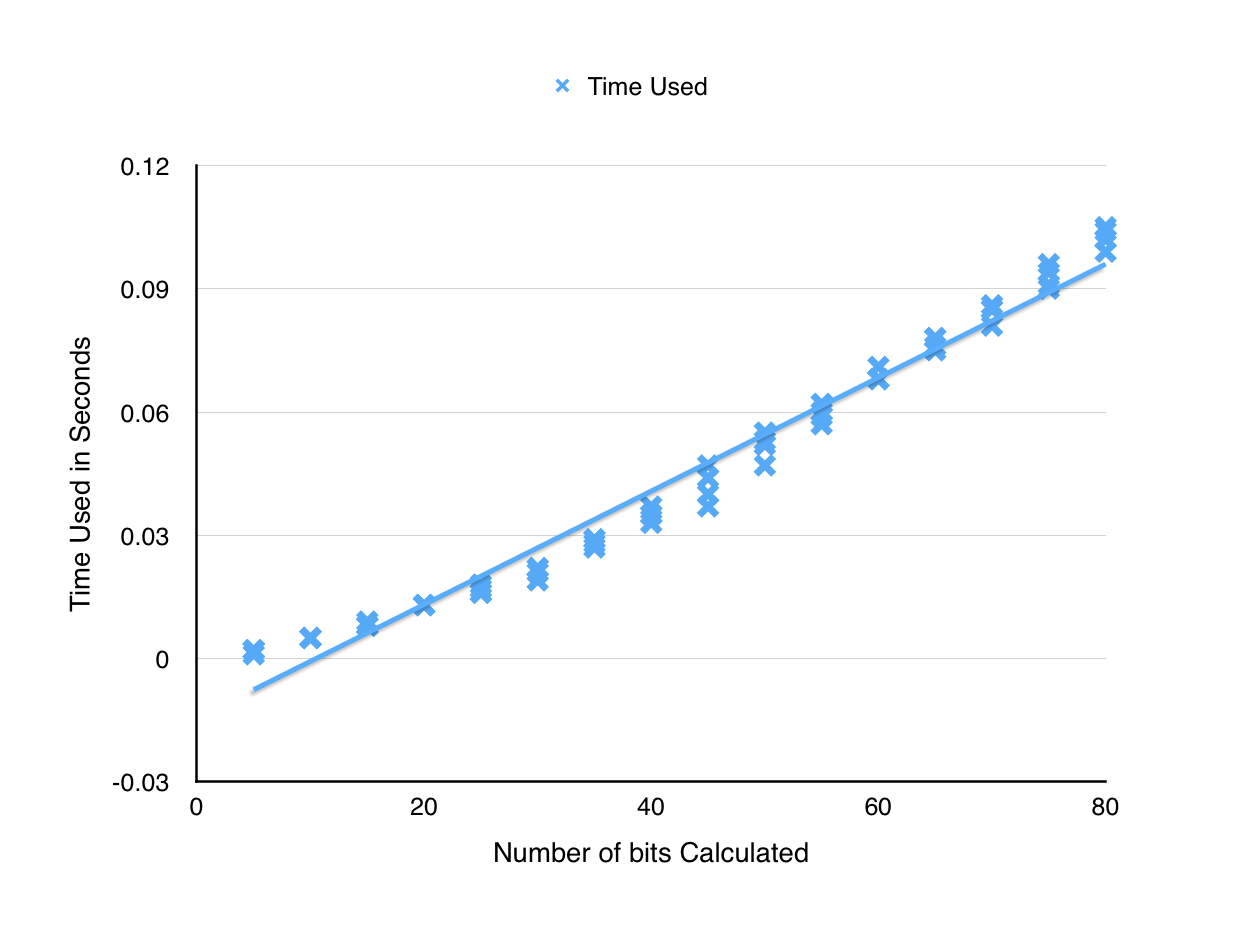
\includegraphics [width=\textwidth] {addres}



\subsection {Multiplication}
Recall the equation 3.1,
\begin{equation}
\begin{split}
A*B=(int1+frac1)*(int2+frac2)\\
=int1*int2+int1*frac2+int2*frac1+frac1*frac2
\end{split}
\end{equation}
Here the three addition in the result is actually two Exreal number addition, since we combine two terms $int1*int2$ and $frac1*frac2$ as one Exreal $R(int1*int2, frac1*frac2)$. \\
We evaluate the complexity part by part in the equation. Let's say that $int1$ has $i_{1}$ bit in binary and $int2$ has $i_{2}$ bit in binary. Thus base on section 3.1.4, calculating $int1*frac2$ and $int2*frac1$ to the nth bit is equivalent to calculating $i_{1}$ / $i_{2}$ Exreal addition to the nth bit. Using the result from 4.2.1, then $int1*frac2$ and $int2*frac1$ has a complexity of $\mathcal{O}(i_{1}*n)$ and $\mathcal{O}(i_{2}*n)$ respectively.\\  
For the $frac1*frac2$ part, we generate a lazy list of Exreals and add them together. Each of the Exreals would take linear time to generate,  thus the complexity is equivalent to doing $(n+2)$ Exreal addition and it has a complexity of $\mathcal{O}((n+2)*n) * \mathcal{O}(n)= \mathcal{O}(n^{3})$. And the integer part multiplication takes $\mathcal{O}(i_{1}*i_{2})$ time. Thus the overall complexity would take
\begin{equation}
\begin{split}
(\mathcal{O}(n^{3}) + \mathcal{O}(i_{1}*i_{2})) + \mathcal{O}(i_{1}*n) + \mathcal{O}(i_{2}*n) =\\ 
\mathcal{O}(n^3) + \mathcal{O}((i_{1}+i_{2}) * n) + \mathcal{O}(i_{1}*i_{2})).  
\end{split}
\end{equation}
When n is large and $i_1$, $i_2$ are small, then the complexity can also be considered as $\mathcal{O}(n^3)$\\
But in reality the program runs at an extremely slow speed. We use 3 different multiplication examples and calculate them up to 1,2,3 bits respectively. The results shown as below.

\begin{longtable}{| l | l | l |}
	\hline
    	Number of Bits Calculated & Time used in Seconds & Test Case \\ \hline
	1 & 0.924 & 0.5*0.25 =0.125 \\ \hline
	2 & 219.455 & \\ \hline
	3 & $>$7200 & \\ \hline
	1 & 0.086 & 0.62*0.53 = 0.3286\\ \hline
	2 & 28.072 & \\ \hline
	3 & 7157.312 & \\ \hline
	1 & 1.462 & 0.95*0.8 = 0.76 \\ \hline
	2 & 465.264 & \\ \hline
	3 & $>$7200 & \\ \hline
\end{longtable}






\section{Sierpinski Space and complexity}
\subsection{Sierpinski Space Complexity}

Due to the semi-decidable nature of the Sierpinski Space datatype, we can make any functions, that takes any arbitrary input and outputs Sierpinski Space, become a linear time function\cite{pauly-kawamura-arxiv}. Consider an arbitrary computable function $f(x)$ such that f maps some $x$ into the Sierpinski Space.  Here $x$ is not necessarily an Exreal number, $x$ can be any data types, such as open sets or compact sets etc. We can construct a linear time computable function $g(x)$ that is equivalent to $f(x)$. \\
$g(x)$ is defined as : \\
At any given time t, $g(x)$ is asked to produce a bit of result, then $g(x)$ simulates $f(x)$ up until time t and save the current state for continuation. If $f(x)$ has output any result up until time t, then $g(x)$ returns the same result and ask f about the next bit result. If $f(x)$ outputs nothing then $g(x)$ adds a false to the result.\\
$g(x)$ and $f(x)$ are equivalent since if $f(x)$ will ever output any true at time t that makes the result maps to $\top$ then so will $g(x)$ at time t. Otherwise $g(x)$ would constantly return false as well. Thus it is meaningless to analyse the complexity of any functions that outputs Sierpinski Space. 


\subsection{Inverse function calculator performance}
Since it is impossible to analyse the complexity of Sierpinski Space functions in a meaningful way, we would use Timer structure to estimate the time cost of the inverse function calculator. Here we test the performance of the inverse function of $x+x$ which give us the divide by 2 function in Exreal using Timer structure. We use the test code as shown in \textbf{Chapter 3.8.2} and calculate 3 test cases result up to 1,2,3,4,5,6 bits respectively. \\
The three test cases are $0.5/2 = 0.25$, $0.75/2 = 0.375$, $0.875/2 = 0.4375$. 

\begin{longtable}{| l | l | l |}
	\hline
    	Number of Bits Calculated & Time used in Seconds & Test Case \\ \hline
	1 & 1.193 & 0.5/2 =0.25 \\ \hline
	2 & 4.881 & \\ \hline
	3 & 15.813 & \\ \hline
	4 & 40.429 & \\ \hline
	5 & 93.489 & \\ \hline
	6 & 200.784 & \\ \hline
	1 & 1.170 & 0.75/2 =0.375 \\ \hline
	2 & 5.971 & \\ \hline
	3 & 19.338 & \\ \hline
	4 & 51.158 & \\ \hline
	5 & 120.058 & \\ \hline
	6 & 256.660 & \\ \hline
	1 & 1.249 & 0.875/2 =0.4375 \\ \hline
	2 & 5.964 & \\ \hline
	3 & 21.602 & \\ \hline
	4 & 57.564 & \\ \hline
	5 & 139.377 & \\ \hline
	6 & 305.312 & \\ \hline
\end{longtable}

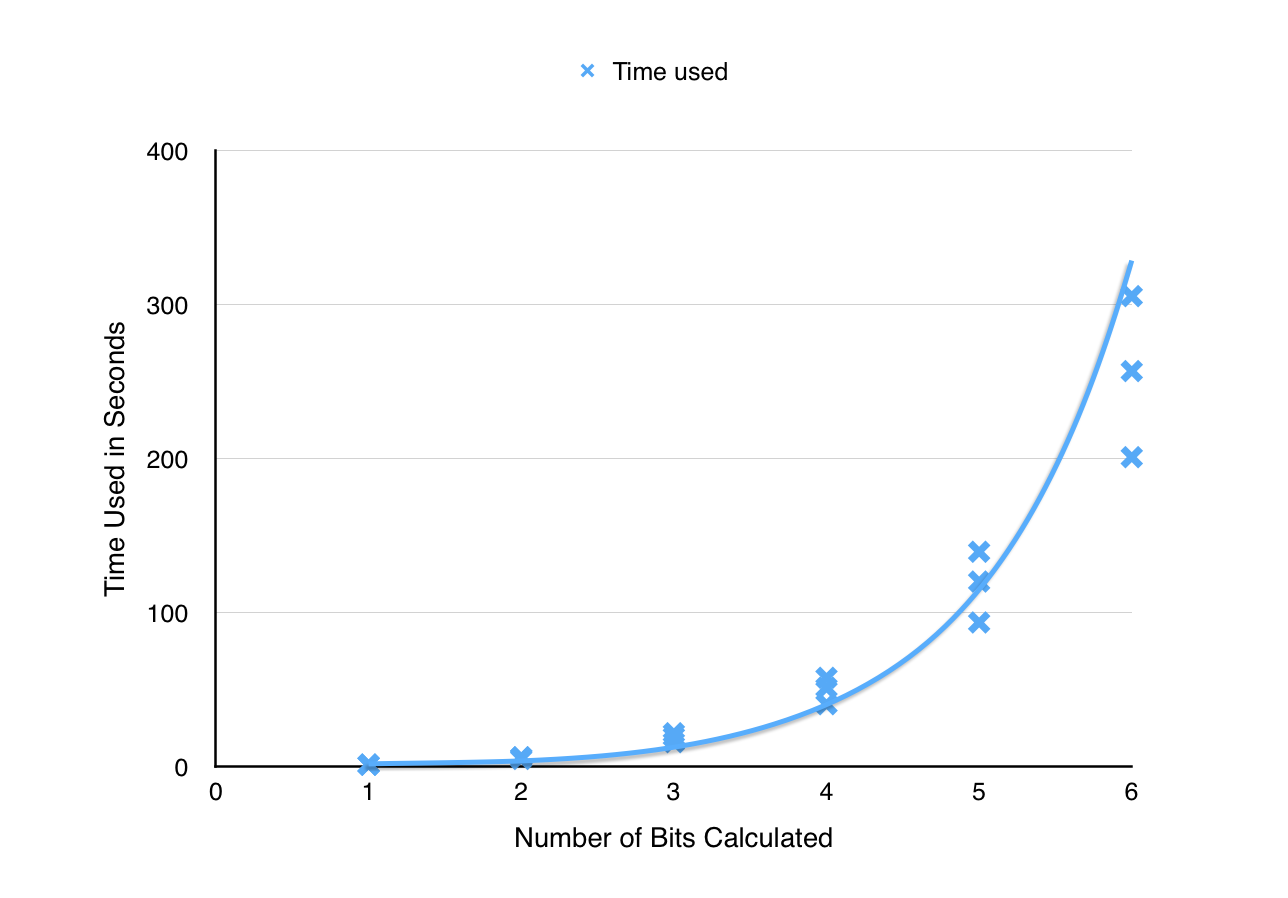
\includegraphics [width=\textwidth] {invres}

The result indicates that the inverse function calculator for $f(x) = x+x$ has an exponential complexity with an exponent between 2 and 3.


\section{Functionality}
As discussed in introduction, this project has a different approach then other exact real packages available. The inverse function calculator allow us to implement certain functions in Exact Real very easily. Such as the square root function might not be easy to implement directly. But using the inverse function calculator, it can be implemented using the exact code for divide by 2 function, except changing the addition into multiplication, like below, 

{\setstretch{0.8}
\begin{verbatim}
> fun exr_sqrt y = inverse (fn x=> (rmult x x) ) y;
val exr_sqrt = fn: exreal -> exreal
\end{verbatim}
} 

The project limitation would be the performance, it would took a very long time before the square root function can return any meaningful result but the package do provide us with an extremely easy way of implementing the function.
Thus despite the rather poor performance of the package, the extendability is huge.



\chapter{Conclusion}

In this project, I have achieved the primary original goals, developing an Exact real package in ML. The project started with researching in current exact real packages and different real representations. Then the signed digit representation is chosen for the project. And the exreal data structure is then implemented with basic arithmetic operation implemented as well. Then using the idea of synthetic topology, topological data structure such as open/closed set and compact set on exact real number is implemented. A very important application of the project, an abstract inverse function calculator is implemented and tested. Then I did a complexity analysis and performance test on the developed datatype. 

\section{Lessons Learned}

\begin{itemize}
\item Do not get too ambitious when designing the goal of the project. In the original project proposal, one of the goal is to have a performance comparison between my developed exact real package with the current existing iRRAM package. This turn out to be not realistic. The performance of the designed exact real package is no where near iRRAM.
\end{itemize}


\section{Future Work}

If more time were given, an abstract method of integrating continuous functions on Exreal can be implemented. Integration can be achieved in a synthetic framework is shown in \emph{Computable Stochastic Processes} by Pieter Collins \cite{collins4}.
Also there is room for a performance improvement as well. 


\cleardoublepage

%%%%%%%%%%%%%%%%%%%%%%%%%%%%%%%%%%%%%%%%%%%%%%%%%%%%%%%%%%%%%%%%%%%%%
% the bibliography

\addcontentsline{toc}{chapter}{Bibliography}
\bibliography{refs}
\cleardoublepage

%%%%%%%%%%%%%%%%%%%%%%%%%%%%%%%%%%%%%%%%%%%%%%%%%%%%%%%%%%%%%%%%%%%%%
% the appendices
\appendix

\chapter{Key Source Code}

\section{Exreal Datatype}
{\scriptsize\verbatiminput{exreal.txt}}

\section{Sierpinski Space}
{\scriptsize\verbatiminput{sierp.txt}}

\section{Open/Closed Set}
{\scriptsize\verbatiminput{openclose.txt}}

\section{Compactness}
{\scriptsize\verbatiminput{compact.txt}}

\section{Admissibility}
{\scriptsize\verbatiminput{adm.txt}}



\cleardoublepage

\chapter{Project Proposal}

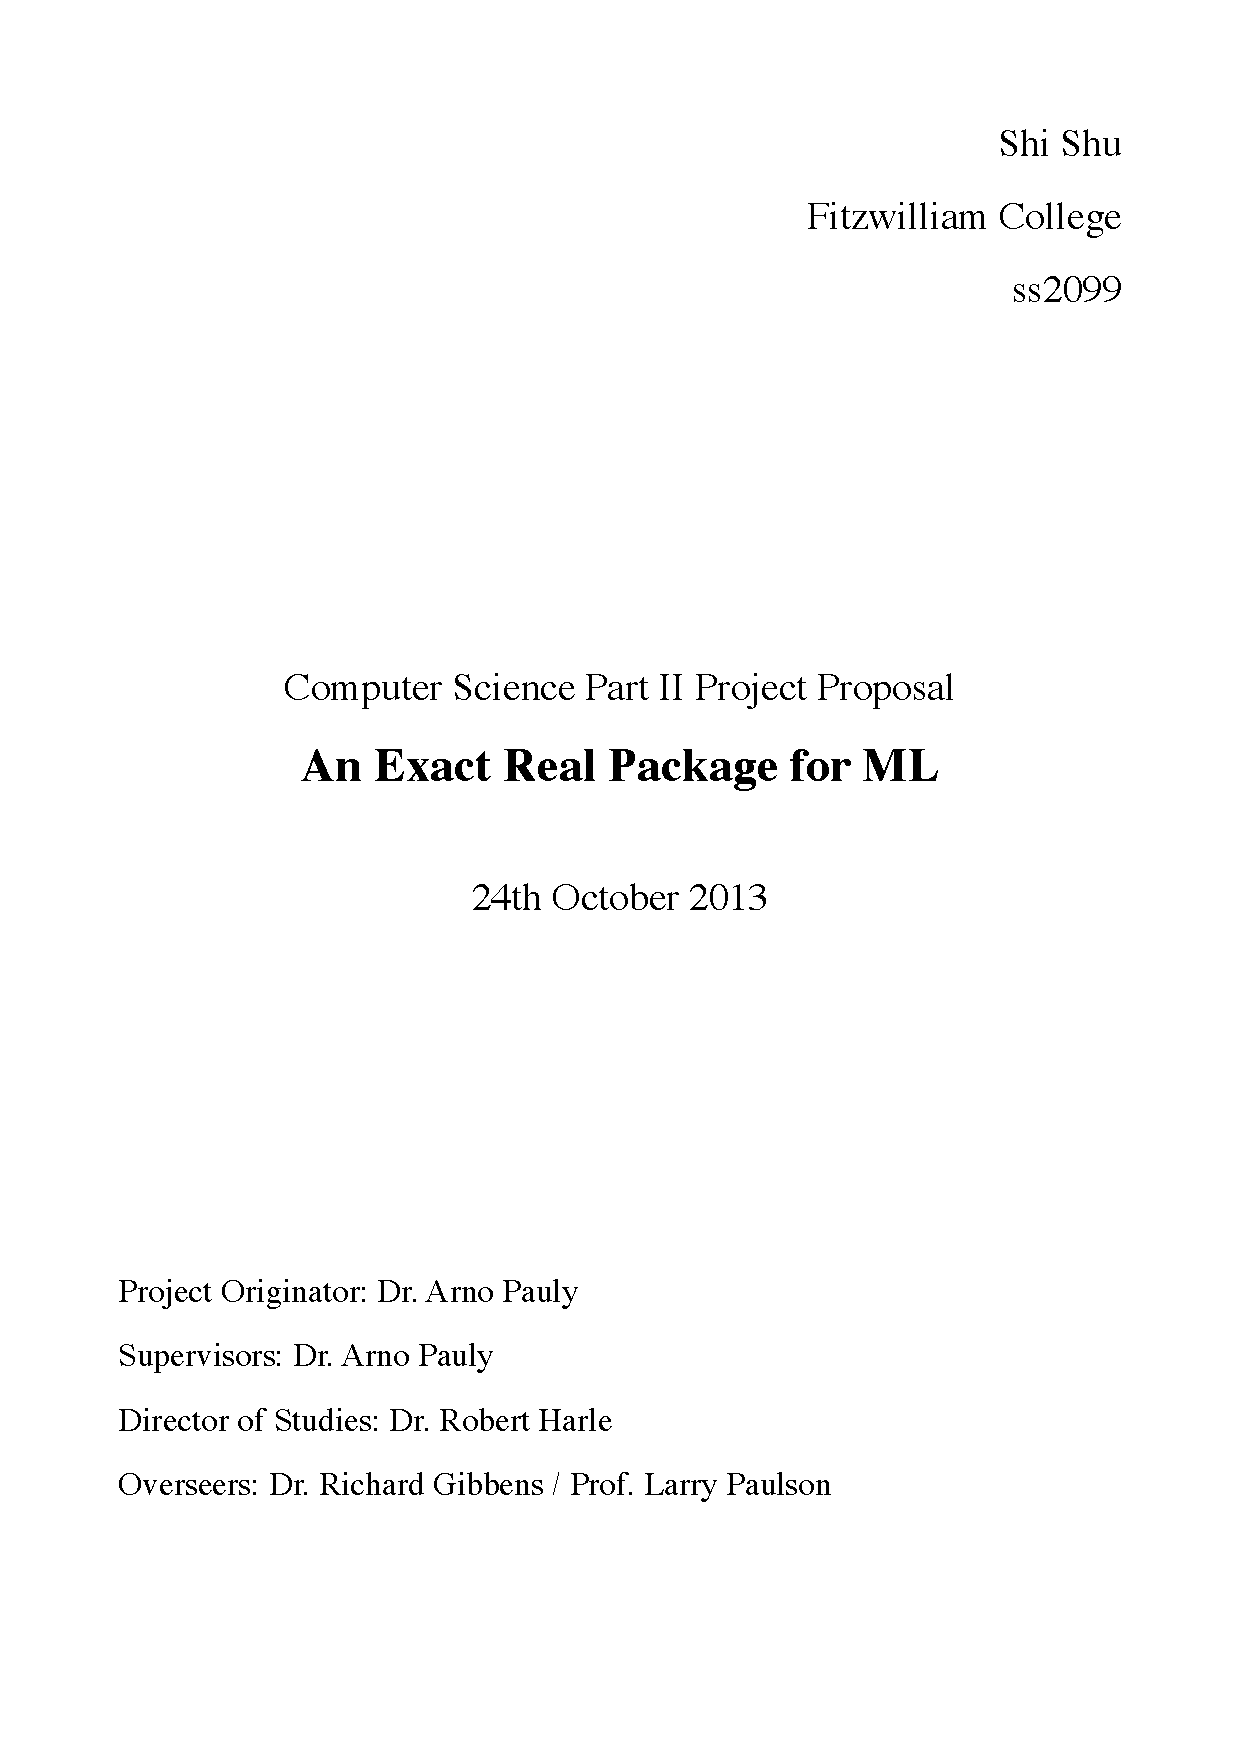
\includepdf[pages=-]{proposal.pdf}

\end{document}
